\section{Problem Modeling}
\label{sec:model}

For a prescribed number $N$ of identical turbines with rotor radius $R$ (diameter $D=2R$), the $n=2N$ coordinates of the layout $\mathbf X=(x_1,y_1,\ldots,x_N,y_N)$ are optimized to maximize the expected farm power, i.e., to minimize the wake loss, under the Jensen wake model~\cite{Jensen1983,Katic1986} and the power curve of~\cite{Kusiak2010}. The wind direction $\theta$ has the probability density $p_\theta$, and for each direction the wind speed $s$ follows a Weibull density $p_s(s;\zeta,\psi)$ with shape $\zeta(\theta)$ and scale $\psi(\theta)$. Here $\theta$ is the direction \emph{towards} which the wind blows, counter-clockwise from east (Fig.~\ref{fig:S-farm}); the meteorological directions $\theta_{\rm met}$ of Horns Rev~1 and IEA37 (wind \emph{from}, clockwise from north) are converted by $\theta=270^\circ-\theta_{\rm met}$. Two constraints apply: all turbine pairs satisfy $\ell_{ij}=\lVert(x_i-x_j,\,y_i-y_j)\rVert_2\ge\ell_{\min}=4D=8R$, as in~\cite{Kusiak2010,Bansal2017}, and the farm is circular, $x_i^2+y_i^2\le r^2$, with $r=500$, 750 or 1000~m. Figs.~\ref{fig:S-farm}--\ref{fig:S-halfcone} show the geometry; the sections below define the wind model, the wake and power models, the objective and the constraint handling that all optimizers of Section~\ref{sec:prelim} share.

\begin{figure}[!t]
\centering
\begin{minipage}[b]{0.40\textwidth}
\centering
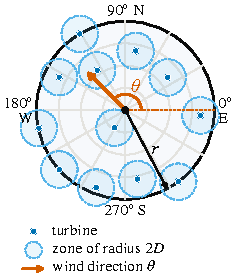
\includegraphics[width=\linewidth]{figures_final/fig_wind_farm.pdf}
\caption{Circular wind farm of radius $r$ and wind direction $\theta$ (blowing towards, counter-clockwise from east). The points show, for illustration only, a 12-turbine layout of an earlier version of this study (LX-SSA-VNS, $r=750$~m, Data Set~I); the discs have radius $2D$, so two discs touch when their turbines are exactly $\ell_{\min}=4D$ apart.}
\label{fig:S-farm}
\end{minipage}\hfill
\begin{minipage}[b]{0.54\textwidth}
\centering
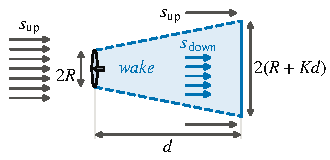
\includegraphics[width=0.88\linewidth]{figures_final/fig_wake_model.pdf}
\caption{Jensen top-hat wake behind a rotor of radius $R$ (schematic). At the downstream distance $d$ the wake has the width $2(R+Kd)$ and the uniform speed $s_{\text{down}}<s_{\text{up}}$.}
\label{fig:S-wake}
\par\medskip
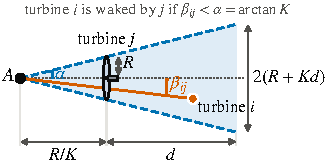
\includegraphics[width=0.88\linewidth]{figures_final/fig_half_cone.pdf}
\caption{Wake half cone of turbine $j$ ($K$ exaggerated): virtual vertex $A$ at $R/K$ upstream of the rotor, half-angle $\alpha=\arctan K$; turbine $i$ is waked by $j$ if $\beta_{ij}<\alpha$.}
\label{fig:S-halfcone}
\end{minipage}
\end{figure}

\subsection{Wind Model and Direction Discretization}
\label{sec:wind}
In every direction the wind speed is Weibull distributed,
\begin{equation}
p_s(s;\zeta,\psi)=\frac{\zeta}{\psi}\Bigl(\frac{s}{\psi}\Bigr)^{\zeta-1}\exp\Bigl[-\Bigl(\frac{s}{\psi}\Bigr)^{\zeta}\Bigr],\qquad \Pr(S>s)=\exp\Bigl[-\Bigl(\frac{s}{\psi}\Bigr)^{\zeta}\Bigr],\qquad s\ge0 .
\label{eq:weibull}
\end{equation}
The benchmark rose is piecewise constant: $N_\theta=24$ direction bins $[15(l-1),15l)^\circ$, $l=1,\ldots,24$, with probability $p_l$, shape $\zeta=2$ and scale $\psi_l$ (Table~\ref{tab:S-wind}). Data Set~I is nearly unidirectional ($\psi=13$~m/s in all bins; 80\% of the probability in bins 6 and 7, i.e., wind from 165$^\circ$ to 195$^\circ$), Data Set~II is a broad rose with scales from 2.6 to 10~m/s and its highest probability in bin~13. The Horns Rev~1 block uses a measured 12-sector Weibull rose evaluated in 5$^\circ$ bins, and IEA37 Case Study~1 16 directions at one speed (Section~\ref{sec:setup-beyond}).

\begin{table}[!t]
\centering
\caption{Wind Data Sets I and II of the benchmark~\cite{Kusiak2010,Bansal2017}: probability $p_l$ of direction bin $l$ ($[15(l-1),15l)^\circ$, direction the wind blows towards, counter-clockwise from east) and Weibull scale $\psi$ (m/s); $\zeta=2$ in all bins. The most probable bin is $l=7$ (wind from 165$^\circ$--180$^\circ$ in the meteorological convention) for Data Set~I and $l=13$ (wind from 75$^\circ$--90$^\circ$) for Data Set~II.}
\label{tab:S-wind}
\scriptsize\setlength{\tabcolsep}{3.2pt}
\begin{tabular}{l*{12}{c}}
\toprule
Bin $l$ & 1 & 2 & 3 & 4 & 5 & 6 & 7 & 8 & 9 & 10 & 11 & 12 \\
\midrule
DS I: $p_l$ ($\psi=13$) & 0.000 & 0.010 & 0.010 & 0.010 & 0.010 & 0.200 & 0.600 & 0.010 & 0.010 & 0.010 & 0.010 & 0.010 \\
DS II: $\psi$ & 7.0 & 5.0 & 5.0 & 5.0 & 5.0 & 4.0 & 5.0 & 6.0 & 7.0 & 7.0 & 8.0 & 9.5 \\
DS II: $p_l$ & 0.0002 & 0.0080 & 0.0227 & 0.0242 & 0.0225 & 0.0339 & 0.0423 & 0.0290 & 0.0617 & 0.0813 & 0.0994 & 0.1394 \\
\midrule
Bin $l$ & 13 & 14 & 15 & 16 & 17 & 18 & 19 & 20 & 21 & 22 & 23 & 24 \\
\midrule
DS I: $p_l$ ($\psi=13$) & 0.010 & 0.010 & 0.010 & 0.010 & 0.010 & 0.010 & 0.010 & 0.010 & 0.010 & 0.010 & 0.010 & 0.000 \\
DS II: $\psi$ & 10.0 & 8.5 & 8.5 & 6.5 & 4.6 & 2.6 & 8.0 & 5.0 & 6.4 & 5.2 & 4.5 & 3.9 \\
DS II: $p_l$ & 0.1839 & 0.1115 & 0.0765 & 0.0080 & 0.0051 & 0.0019 & 0.0012 & 0.0010 & 0.0017 & 0.0031 & 0.0097 & 0.0317 \\
\bottomrule
\end{tabular}
\end{table}
% verified: values = analysis/wflop_model.py (DS1_W, DS1_PSI, DS2_PSI, DS2_W; k = 2); bins 6+7 of DS I: 0.2+0.6 = 0.8, towards 75-105 deg = from 165-195 deg

\emph{Why the direction discretization matters.} The objective evaluates the wake only at the bin centres $\bar\theta_l=15l-7.5^\circ$, i.e., it treats the rose as 24 discrete winds. A top-hat wake is narrow: by the half-cone geometry (Fig.~\ref{fig:S-halfcone}), turbine $j$ wakes a turbine $i$ at the distance $\rho\ge R/K$ only for wind directions within an interval of width $2[\alpha+\arcsin(R/(\rho\sqrt{1+K^2}))]$ around the direction from $j$ to $i$. With the benchmark values ($K=0.075$, $R=38.5$~m; $\alpha=4.29^\circ$, $R/K=513$~m) this width falls below the bin spacing of 15$^\circ$ for $\rho>685$~m and tends to $2\alpha=8.6^\circ$ for distant pairs. Such a pair can be placed so that no bin centre lies in its wake interval, and its wake then does not enter the objective, although it exists for the directions between the centres. With bins of 5$^\circ$ or finer, every such interval contains a bin centre. Optimized layouts exploit these gaps: re-evaluated with 1$^\circ$ sub-bins that keep the Weibull parameters of their 15$^\circ$ bin, the mean wake loss of PSO-VNS rises from \NFLossPSOVNSFifteen\% to \NFLossPSOVNSOne\%, and the rise is largest for PSO and the VNS-based methods (Section~\ref{sec:robustness}). All results therefore hold for the discretized roses of the benchmark and of Horns Rev~1; Section~\ref{sec:robustness} reports which conclusions survive a 1$^\circ$ rose.
% verified (numerically with analysis/wflop_model.jensen_deficits on a 0.001-deg grid): waked width of a pair rho apart = 2(alpha + arcsin(R/(rho sqrt(1+K^2)))) exactly for rho >= R/K (rho = 600: 15.915 deg; 1000: 12.979; 2000: 10.779); width = 15 deg at rho = 685.4 m; alpha = arctan 0.075 = 4.289 deg; R/K = 513.3 m; 2 alpha = 8.58 deg > 5 deg. For rho < R/K the non-physical upstream deficit widens the interval further.
% CHECK-DIR [F03]: loss rise of every method, PSO-VNS 1.322 -> 2.335; [F05]: VNS-based methods and PSO rise most

\subsection{Wake Effect Model}
In the Jensen model (Figs.~\ref{fig:S-wake} and~\ref{fig:S-halfcone}), the wake of turbine $j$ is a half cone with half-angle $\alpha=\arctan K$ (wake-spreading constant $K$), and its virtual vertex lies $R/K$ upstream of the rotor. With $u_{ij}=(x_i - x_j)\cos\theta + (y_i - y_j)\sin\theta + R/K$ and the lateral offset $v_{ij}=-(x_i - x_j)\sin\theta + (y_i - y_j)\cos\theta$, turbine $i$ lies in the wake if $\beta_{ij}=\cos^{-1}\!\bigl(u_{ij}/\sqrt{u_{ij}^2+v_{ij}^2}\bigr)<\alpha$, i.e., if its hub lies inside the cone. Its downstream distance is $d_{ij}=\lvert u_{ij}-R/K\rvert$, and with the thrust coefficient $C_T$ the velocity deficit is
\begin{equation}
    \Delta_{ij} = 1-\frac{s_{\text{down}}}{s_{\text{up}}}=\frac{1 - \sqrt{1 - C_T}}{\left(1 + K d_{ij}/R\right)^2}.
    \label{eq:deficit}
\end{equation}
The numerator is the deficit just behind the rotor given by actuator-disc momentum theory, and the factor $R^2/(R+Kd_{ij})^2$ spreads it over the growing wake cross-section (Fig.~\ref{fig:S-wake}). With the benchmark values $C_T=0.8$ and $K=0.075$, a turbine directly $\ell_{\min}=308$~m behind another loses 21.6\% of the wind speed, and one 770~m ($10D$) behind loses 8.8\%.
% verified: (1-sqrt(0.2))/(1+0.075*308/38.5)^2 = 0.2159; (1-sqrt(0.2))/(1+0.075*770/38.5)^2 = 0.0884
As in~\cite{Kusiak2010}, this top-hat wake is tested at the hub center only, so the deficit jumps at the cone edge, and it also reaches a turbine less than $R/K$ \emph{upstream} of $j$ near its axis (between $A$ and the rotor in Fig.~\ref{fig:S-halfcone}; non-physical, kept for comparability with the published results). The deficits are combined by the root-sum-square rule,
\begin{equation}\label{eq5}
\Delta_i(\theta) = \Bigl( \textstyle\sum_{j \ne i,\ \beta_{ij} < \alpha} \Delta_{ij}^2 \Bigr)^{1/2} .
\end{equation}
As $C_T$ is constant (which overstates the deficits above rated speed), the local wind speed in a direction bin is the free-stream speed times $1-\Delta_i(\theta)$, a Weibull variable with shape $\zeta(\theta)$ and scale $\psi_i(\theta)=\psi(\theta)[1-\Delta_i(\theta)]$. Because of the hub-center in-wake test, the objective jumps where a hub crosses a cone edge in one of the evaluated directions; this is why the local search of VNS is derivative-free (Section~\ref{sec:vns}) and why finite-difference gradients handicap MS-SLSQP.

\subsection{Power Model and Expected Energy}
\label{sec:powermodel}
\label{sec:S-power}
The power curve of the Kusiak--Song benchmark~\cite{Kusiak2010} is $f(s)=0$ for $s<s_{\text{cut-in}}$, $f(s)=\lambda_1 s+\lambda_0$ for $s_{\text{cut-in}}\le s\le s_{\text{rated}}$ and $f(s)=P_{\text{rated}}$ above, with $s_{\text{cut-in}}=3.5$~m/s, $s_{\text{rated}}=14$~m/s, $P_{\text{rated}}=1500$~kW, $\lambda_1=140.86$ and $\lambda_0=-500$. We use it as published: it is slightly negative just above the cut-in speed ($-7.0$~kW at 3.5~m/s, zero at 3.55~m/s), jumps from 1472 to 1500~kW at the rated speed and has no cut-out speed. The expected power of turbine $i$,
\begin{equation}\label{eq8}
E(P_i) = \int_0^{360} p_\theta(\theta) \int_0^{\infty} f(s)\,
       p_s\bigl(s; \zeta(\theta), \psi_i(\theta)\bigr) \, ds \, d\theta ,
\end{equation}
is evaluated, as in~\cite{Kusiak2010}, by a Riemann sum. The direction axis is divided into bins $\theta_0 = 0^\circ, \theta_1, \ldots, \theta_{N_\theta} = 360^\circ$ with probabilities $p_l$, and the speed range between $s_{\text{cut-in}}$ and $s_{\text{rated}}$ into $N_s$ bins $s_0 = s_{\text{cut-in}}, s_1, \ldots, s_{N_s} = s_{\text{rated}}$ (benchmark: $N_\theta=24$ bins of 15$^\circ$ and $N_s=21$ bins of 0.5~m/s). With the bin centres $\bar\theta_l=(\theta_{l-1}+\theta_l)/2$ and the Weibull survival function $W_i(s,\theta)=\exp\{-[s/\psi_i(\theta)]^{\zeta(\theta)}\}$ of the local speed,
\begin{equation}
\begin{split}
E(P_i) ={}& \sum_{l=1}^{N_\theta} (\theta_l - \theta_{l-1})\, p_l \Bigg\{ P_{\text{rated}}\, W_i(s_{\text{rated}},\bar\theta_l)
+\lambda_1 \sum_{q=1}^{N_s} \frac{s_{q-1} + s_q}{2}\left[W_i(s_{q-1},\bar\theta_l)-W_i(s_q,\bar\theta_l)\right]\\
&+ \lambda_0 \left[W_i(s_{\text{cut-in}},\bar\theta_l)-W_i(s_{\text{rated}},\bar\theta_l)\right] \Bigg\}.
\end{split}
\label{eq:S-power}
\end{equation}
The first term is the rated power times the probability of a local speed above $s_{\text{rated}}$, the second integrates $\lambda_1 s$ by the midpoint rule over the speed bins, and the third adds $\lambda_0$ times the probability of the linear range. Like the earlier studies, we keep the bin-width factor $(\theta_l-\theta_{l-1})$ in degrees. Because all 24 direction bins are $15^\circ$ wide and $\sum_l p_l=1$, the benchmark objective $\sum_i E(P_i)$ is 15 times the expected farm power in kW, and the gross (wake-only) annual energy production of the benchmark is $\mathrm{AEP}\,[\mathrm{MWh}] = (\text{objective}/15)\times 8.76$. The wake-free benchmark objective of one turbine, $E_{\rm ideal}$, is~\eqref{eq:S-power} with $\psi_i=\psi$; for Data Set~I, $E_{\rm ideal}=14{,}045.74$, which corresponds to 936.38~kW (a capacity factor of 62\%, far above real sites) or 8,202.7~MWh/yr.
% verified: 14045.74/15 = 936.38 kW; 936.38/1500 = 0.624; 936.38*8.76 = 8202.7 MWh (R4 reproduced these from wflop_model.py); N_s = (14-3.5)/0.5 = 21 (wflop_model.expected_power_linear); 140.86*3.5-500 = -6.99; 500/140.86 = 3.55; 140.86*14-500 = 1472.0

\subsection{Optimization Problem and Constraint Handling}
\label{sec:constraints}
With the wake loss $L(\mathbf X)=N E_{\rm ideal}-\sum_{i=1}^{N}E(P_i)$, reported in percent of the wake-free value, $100\,L/(NE_{\rm ideal})$, the problem is
\begin{equation}
\min_{\mathbf X\in[-r,r]^{2N}} L(\mathbf X)\quad\text{s.t.}\quad \ell_{ij}\ge\ell_{\min}\ (1\le i<j\le N),\qquad x_i^2+y_i^2\le r^2\ (1\le i\le N),
\label{eq:wflop}
\end{equation}
which is equivalent to maximizing the expected farm power and hence the AEP: a problem in $2N$ variables ($2N\le30$ on the benchmark) with a discontinuous objective and $N(N-1)/2$ nonconvex spacing constraints.
After every position update, each coordinate is clipped to $[-r,r]$ (box repair; the square, not the circle). The constraints are handled by a penalty on the violations $g^{\rm b}_{i}=x_i^2+y_i^2-r^2$ and $g^{\rm s}_{ij}=\ell_{\min}-\ell_{ij}$; all optimizers except MS-SLSQP minimize the penalized wake loss
\begin{equation}
\begin{split}
F_p(\mathbf X)={}&\Bigl(N E_{\rm ideal}-\sum_{i=1}^{N}E(P_i)\Bigr)+\sum_{i:\,g^{\rm b}_i>0}\bigl(1+\mu g^{\rm b}_i\bigr)^2\\
&+\sum_{i<j:\,g^{\rm s}_{ij}>0}\bigl(1+\mu g^{\rm s}_{ij}\bigr)^2,\qquad \mu=10^{10},
\end{split}
\label{eq:penalty}
\end{equation}
whose first term is the wake loss $L(\mathbf X)$ reported in our tables. Any violation above about $4.6\cdot10^{-8}$ (m or m$^2$) makes the penalty exceed any possible wake loss, so comparing $F_p$ values is, up to smaller violations, a feasibility-first rule (feasible before infeasible, then wake loss or total penalty). This penalty scaling ($g^{\rm b}_i$ in m$^2$, $g^{\rm s}_{ij}$ in m) favours infeasible layouts inside the farm with turbines too close, or with a turbine clipped to the box near a tangent point $(\pm r,y_i)$, where $g^{\rm b}_i=y_i^2$ is second order in $y_i$. MS-SLSQP minimizes the wake loss under explicit constraints. A final layout counts as feasible if $\ell_{ij}\ge\ell_{\min}$ and $\sqrt{x_i^2+y_i^2}\le r$ hold within $10^{-6}$~m (Section~\ref{sec:setup}), a looser tolerance than the penalty's.
% verified (R3-11): largest benchmark wake loss < 15 x 14045.74 = 2.107e5 (plus the small negative part of f); (sqrt(2.2e5)-1)/1e10 = 4.6e-8
% CHECK-DIAG [D06]/[D21]: old-setting infeasible finals (1e-6 m rule) mostly spacing-only; boundary violations = turbine with a coordinate on the box bound (tangent-point pinning); numbers in 04 sec:pso
